%%% Local Variables:
%%% TeX-master: "AbilityMaster"
%%% End:%%% Local Variables:
%%% TeX-master: "master"
%%% End:

\chapter{The Potentive Inference --- Attribution and Witnessing}
\label{cha:potent-infer-attr}

\begin{note}[Overview]
  In this section we examine the type of ability statements used in some detail.

  \begin{itemize}
  \item The potentive inference.
  \item \AR{} and \WR{}.
  \item Differences between \AR{} and \WR{}.
  \item (Possibly) further notes on \WR{}.
  \end{itemize}
\end{note}

\section{Potentive entailment}
\label{sec:potentive-entailment}

{
  \color{red}
  Replace `inference' with `entailment', as I don't want to focus solely on the use of this in reasoning.
}

\begin{note}[Overview]
  We being with a general overview of the potentive inference.
  After establishing the basics, we then turn to the two ways outlined.
  \AR{} and \WR{}.
\end{note}

\begin{note}[Potentive inference]
  In order for there to be potential that \(\phi\) is the case, \(\psi\) must be the case.

  Potentive = adjective of potential.
\end{note}

\begin{note}[Examples]
  Simple instances of the potentive inference involve factive verbs, in which the relevant fact holds independently of whether the verb is witnessed.
  \begin{itemize}
  \item Sam has the ability to show that \(19\) is a prime number.
  \item Taylor has the ability to derive Transposition.
  \item Jesse has the ability to \dots
  \end{itemize}

  Note also that the verb does not need to involve some reasoning.
  \begin{itemize}
  \item Corey has the ability to see there is a zebra in the pen.
  \item X has the ability to hear that there is a waterfall nearby.
  \end{itemize}
\end{note}

\begin{note}[Breaking things down]
  \begin{quote}
    \emph{S} has the ability to \emph{V} that \(\phi\).
  \end{quote}
  We have
  \begin{itemize}
  \item Some result of the verb.
  \item A verb.
  \item Modal, ability.
  \item Copula.
  \item An agent.
  \end{itemize}
  As noted, potentive inference works because certain things must be the case in order for there to be a potential event.
\end{note}

\begin{note}[Understanding of the inference]
  The key parts of the inference are the relation between ability and the verb.

  Certain things must be true in order for the verb.
  These are the things which are obtained by the potentive inference.

  In the case of reasoning, note that there must be premises from which the agent works from.
\end{note}

\begin{note}[Observation in terms of propositional/doxastic]
  One way to view this is that if the agent has information, then the agent may infer that they have propositional support for the conclusion which may be turned in to doxastic support.
\end{note}

\begin{note}[Some formal stuff]
  \[\exists e(\text{Able}(s,e) \land (V(e) \land \text{agent} = s \land \text{result}(e) = \phi))\]
  There is some event \(e\), such that \emph{s} is able to bring about, and \(e\) consists of \emph{s} \emph{V}ing with the result that \(\phi\).

  This requires some non-standard existential, but we're not too interested in providing an analysis suitable for semantics.

  Still, there's nothing too special about the position of the existential.
  Understand ability as relating the agent directly to an event.
  Alternative it to take a truth value.
  \((\text{Able}(s,\exists (V(e) \land \text{agent} = s \land \text{result}(e) = \phi))\).

  Close to having a possible world with \(\phi\) and accessibility relation.
  Interpret the non-standard existential in this way, if it helps.
  There is some possible world and some event in that world, such that the agent at the world of evaluation is able to perform the event witnessed at the possible world.

  In both cases, it's the role of the event.

  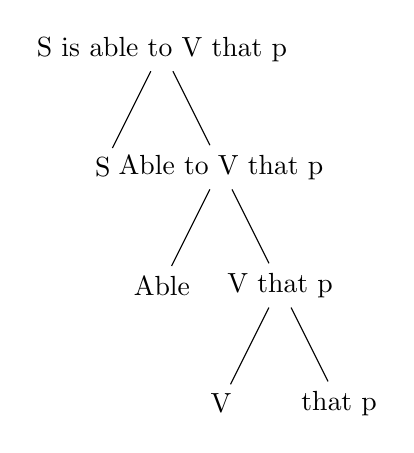
\begin{tikzpicture}[
    ]
    \node{S is able to V that p}
    child {node {S}}
    child {node {Able to V that p}
      child {node {Able}}
      child {node {V that p}
        child {node {V}
        }
        child {node {that p}
        }
      }
    };
  \end{tikzpicture}

  Take some arbitrary witnessing event.
  If \(\psi\) follows from the (arbitrary) witnessing event, then we have an instance of the potentive inference.
\end{note}

\begin{note}[Expanding the event]
  The description of the witnessing event given is minimal.
  Still, simply add in more detail as desired.
\end{note}

\begin{note}[Specific abilities]
  Applies to specific abilities, as the inference appeals to a witnessing event.
  Analogue holds with respect to general abilities.

  General example:
  \begin{itemize}
  \item Sam has the ability to reason with the rules of chess.
  \end{itemize}
  Infer that there is a body of rules governing chess.
  If there are no rules governing chess, then the agent does not have the ability to reason with those (non-existing) rules.

  Not an instance of the potentive inference, as this doesn't follow from what is required from a witnessing event.

  Similarly, it may be that there is an entailment from general to specific.
  \begin{itemize}
  \item If general, then specific.
  \end{itemize}
  For example, understand the general ability distributively.
  Again, not an instance of the potentive inference, as this doesn't follow from what is required from a witnessing event.
\end{note}

\begin{note}[Paraphrasing (footnote)]
  Various paraphrases are available.
  \begin{itemize}
  \item Corey can see there is a zebra in the pen.
  \end{itemize}
  `Can' introduces the complexity that the agent may be witnessing.
  For example, we observe an excited look appear on Corey's face as they look into the pen.
  `Ah, Corey can see a zebra in the pen.'
  Corey isn't exited because they have the ability to see a zebra in the pen, rather Corey is excited because they are seeing a zebra.
\end{note}

\begin{note}[Restriction on instances of the potentive inference]
  We're interested in certain examples as the agent has all of the resources required, so to speak.

  To illustrate, place the reasoning examples behind a conditional.
  \begin{itemize}
  \item If you teach Sam \dots [factoring method], then Sam will have the ability to show that \(19\) is a prime number.
  \end{itemize}
  Intuitively, this is the result of assuming that some additional property holds of the agent.
  Hence, \(\alpha(s) \rightarrow \dots\).
  For, \(\alpha(s)\) will allow the attribution of ability to be true.
\end{note}

\begin{note}[Reasoning and premises]
  Important to note is that in cases of reasoning, the potentive inference may be applied to obtain the availability of premises.

  The difference is the role of these premises.
\end{note}

\begin{note}[Moving on to a more detailed understanding]
  How exactly the event works.
\end{note}

\section{\AR{} and \WR{}}
\label{sec:ar-wr}

\begin{note}[Overview]
  Interest is in how potentive entailment is used.

  A clearer understanding of \AR{} and \WR{}.

  The significant difference is with reasoning.
  \AR{} uses (a variation of) the potentive inference to obtain support.
  \WR{} uses information obtained by the potentive inference to obtain support.
\end{note}

\begin{note}[Diagram]
  \begin{figure}[h]
  \begin{subfigure}{.5\textwidth}
    \centering
    \begin{tikzpicture}[
      ->,
      >=stealth',
      % auto,
      node distance=0cm, every text node part/.style={align=center},
      ]

      \node [] (c) at (0,0) {};
      \node [] (d) at (-3,0) {};
      \node [] (e) at (3,0) {};
      \node [] (f) at (0,-2.1) {};

      \node (1) at (0,-.1) {Ability};
      \node (2) at (0,-2) {Conclusion};

      \draw [->] (1.270) to [] node[left] {} (2.90);
    \end{tikzpicture}
    \caption{\AR{}}
    \label{fig:AR:support}
  \end{subfigure}
  % \hfill
  \begin{subfigure}{.5\textwidth}
    \centering
    \begin{tikzpicture}[
      ->,
      >=stealth',
  % auto,
      node distance=0cm, every text node part/.style={align=center},
      ]

      \node [] (c) at (0,0) {};
      \node [] (d) at (-3,0) {};
      \node [] (e) at (3,0) {};
      \node [] (f) at (0,-2.1) {};

      \node (premise) at (0,-.1) {Premise};
      \node (conclusion) at (0,-2) {Conclusion};

      \node (x) at (-2,-1.05) {Ability};
      \draw [->] (1.270) to node[left] (3) {} (2.90);

      \node (4) [left of=3, xshift=-2cm] {}; % {\(\exists f (f\Phi = \psi)\)};
      \draw [-{Circle[open]}, dashed] (x.0) to (premise);
      \draw [-{Circle[open]}, dashed] (x.0) to (conclusion);

    \end{tikzpicture}
    \caption{\WR{}}
    \label{fig:WR:support}
  \end{subfigure}
  \caption{Relations of support for \AR{} and \WR{}}
  \label{fig:ARandWR:support}
\end{figure}
\end{note}

\begin{note}[Examples of support relation]
  The interesting issue is the inaccessibility of the premises.
  However, there are other examples in which the same structure is present, but premises are accessible.
  
  Are there other instances of information being used in this way?

  Plausible that go from appearance to support.

  `You are looking at a dog'.

  Here, the agent can infer from testimony that the animal is a dog.
  On the other hand, the agent can take the information to establish a support relation.
  So, visual perception support that the animal is a dog.

  Or, a little better.
  These are coyote tracks.
  Then, different ways to support presence of coyote.
  One is the information provided.
  The other is the tracks.
\end{note}

\begin{note}[The event]
  Two ways for the potentive inference to function.
  Both \AR{} and \WR{} focus on the witnessing event.

  \emph{V}ing that \(\phi\).
  \begin{itemize}
  \item \(\phi\) must be the case in order for the agent to \emph{V} that \(\phi\).
  \item In order for the agent to have the attribute \dots
  \item \(\phi\) is the result of the agent \emph{V}ing.
  \item As a result of witnessing the ability \dots
  \end{itemize}

  So, \AR{} doesn't consider the relevant witnessing, only what must be the case in order for there to be a witnessing event.
  By contrast, \WR{} focuses on guarantees about what transpires in the witnessing event.
\end{note}

\subsection{\AR{}}
\label{sec:ar}



\subsection{\WR{}}
\label{sec:wr}

\begin{note}[Overview]
  Understanding \WR{}.
\end{note}

\begin{note}[Work backwards for the event]
  Work backwards for the event
\end{note}

\begin{note}[How support works]
  In the case of reasoning, the result will be that the agent has information about premises.
  Here, it is important to note that the agent has `propositional' support for the premises, independent of the ability information.
  So, the agent does not need to appeal to the existence of the event as a premise in obtaining support for the conclusion.
  The only relevant support the agent has is the support for the premises.
\end{note}




\subsection{Distinction between \AR{} and \WR{}}
\label{sec:dist-betw-ar}

\begin{note}[Overview]
  The important difference is what supports the conclusion.

  Here, we suggest that further differences depend on additional commitments.
\end{note}


\begin{note}[Key Issue]
  The key issue is whether the agent obtains support for all the relevant preconditions of witnessing the ability by witnessing.
  And, whatever follows from this, e.g.\ in terms of commitments and so on.

  If so, then anything that follows from \AR{} also follows from \WR{}.
  Conversely, as the agent does not obtain information about how the ability is witnessed, it seems what follows from \WR{} also follows from \AR{}.
\end{note}

\begin{note}[Interesting case]
  Interesting case to think about, in which the agent obtains support for what follows from witnessing, but intuitively not for some other precondition.
  \begin{itemize}
  \item Ability to reason to \(\phi\).
  \end{itemize}
  Inference applies to \(\phi\).
  Inference doesn't seem to apply to reasoning to \(\lnot\phi\) as mistaken.
\end{note}

Understanding of ability is such that there is always a potential witnessing event.

\ref{denied-claim} and~\ref{prem:ni} are universal claims.
\ref{prem:ab} is an existential claim.
\ref{denied-claim} and~\ref{prem:ni} clash in scenarios where the possibility captured in~\ref{prem:ab} is realised.

The collection of~\ref{denied-claim},~\ref{prem:ni}, and~\ref{prem:ab} is in tension.

There is an additional secondary premise:

\begin{note}[Two ways to understand ability and support]
\begin{enumerate}
\item\label{prem:ability} Two ways to obtain conclusion given ability.
  \begin{enumerate}
  \item Attribution.
  \item Witnessing.
  \end{enumerate}
\end{enumerate}

\ref{prem:ability} does not make a claim about any particular use of ability.
As a template, conceptually (or logically) coherent.
If there's a problem, then it's because there are further constraints on understanding of support.
\end{note}